\chapter{Concepts \& Trade-Off}
\setlength{\parindent}{15pt}
\label{ch:conc_trad}

\section{Concepts Generation}
\label{sec:conc_gene}

\section{Trade-Off}
\label{sec:trad}
%Trade-off & Sensitivity

The trade-off performed to finalise the decision on which concept is further developed, will be presented here. This section is but a summary on the trade-off process performed in the Midterm Report \cite{midterm}. The trade criteria and its corresponding weights will be discussed in \autoref{sec:trad_crit_weig}, followed by the actual trade-off in \autoref{sec:fina_trad}. Finally, the sensitivity analysis will be presented in \autoref{sec:sens_anal}.

\subsection{Trade Criteria \& Weights}
\label{sec:trad_crit_weig}

The trade criteria have an important impact on the end results of the trade-off. Choosing a criterion which shows no difference in grade for the concepts will adversely impact the trade-off because it will average the results and decrease diversity. This diversity is what should be aimed for to see a distinct difference between the final grades of the concepts, so that the choice for the final concept will be more clear. The explanation of how each criterion affects each concept and the scoring scored for each concept can be found in the Midterm Report \cite{midterm}. Each concept can score between 0 (bad) and 100 (good).

The first criterion is the performance of the concepts. This criterion has been chosen because there are a lot of requirements on the performance of the aircraft. For this criterion the following elements are examined: the mass, the geometric properties, the endurance, the range and the power required of each concept. The next criterion is the manoeuvrability and stability where a sub-trade-off was performed using the manoeuvrability, stability and control of each concept as criteria. Next, the concepts were analysed on ground handling, taking into account how the concepts can be handled for pre-flight preparations. The fourth criterion is the development risk. This criterion will not be split into sub-criteria and had a look at the feasibility, complexity the available knowledge of the concepts, to assess the risk associated with the development phase. The next criterion is the production cost. This criterion is split into manufacturing costs, material costs, mechanisms costs, power and propulsion costs, and finally cost due to weight influence. This criterion has been chosen due to the set limit of 30k for the production cost, limiting the design  possibilities for the aircraft. Then, the sustainability criterion is taken into account and was split into a manufacturing and noise emission analysis. Finally, the reliability criterion took a look into the reliability of the propulsion subsystem, the control surfaces and the wing subsystem.

Assigning weights to the criteria influences the final grades of the trade-off. If an insignificant criterion is weighed more than a significant criterion, the results will be misleading and the final results might change drastically. Furthermore, it is possible to get biased weights when only one person is responsible for weighing the criteria. Therefore, each member of the team was tasked with filling out a form comparing each criterion to all other ones. The averages of the weights for each criterion were taken. These averages were normalised to ten to get a feel as to how much they score on a scale from one to ten. These normalised scores were then converted into percentages to use for the trade-off. 


\subsection{Final Trade-Off}
\label{sec:fina_trad}

This section will present the results of the final trade-off, which can be seen in \autoref{tab:finaltradeoff}. The outcomes of the trade-off will briefly be discussed to get a grasp as to why the concepts scored as they did. Detailed explanation of the separate criteria scores are the result of extensive research on each criterion, the reasoning behind these scores can be found in the Midterm Report \cite{midterm}. For clarity, the table contains colours to give an overview of the severity of the scores. Five colours have been used in a 30-15-10-15-30 spacing (Red, Orange, Yellow, Light Green, Dark Green). This spacing has been used to show more detail around the average than around the extremes. In the event that the table cannot be viewed in colour, each score has a superscript showing which category it scores: 1 = Red, 2 = Orange, 3 = Yellow, 4 = Light Green, 5 = Dark Green. 

\begin{table}[H]
    \setlength\extrarowheight{5pt}
    \setlength\arrayrulewidth{1pt}
    \centering
    \caption{Final Trade-Off}
    \label{tab:finaltradeoff}
    \begin{tabular}{r|>{\centering}p{2.1cm}|>{\centering}p{1.9cm}|>{\centering}p{1.3cm}|>{\centering}p{1.1cm}|>{\centering}p{0.8cm}|>{\centering}p{0.7cm}|>{\centering}p{0.4cm}|c} 
    \textbf{Concept \rotatebox{90}{\hspace{0.5cm}Criterion}}        & 
    \rotatebox{90}{\textbf{Performance}}                            &
    \rotatebox{90}{\textbf{M\&S}}                                   & 
    \rotatebox{90}{\textbf{Reliability}}                            & 
    \rotatebox{90}{\textbf{Production Cost}}                        & 
    \rotatebox{90}{\textbf{Development Risk}}                       &
    \rotatebox{90}{\textbf{Sustainability}}                         &
    \rotatebox{90}{\textbf{Ground Handling}}                        &
    \rotatebox{90}{\textbf{Outcome}}
    \\\hline
    Tailsitter      &
    \cellcolor[HTML]{FFFF00}50$^{^3}$ &
    \cellcolor[HTML]{FFFF00}46$^{^3}$ &
    \cellcolor[HTML]{FFFF00}50$^{^3}$ &
    \cellcolor[HTML]{FFFF00}50$^{^3}$ &
    \cellcolor[HTML]{00B050}75$^{^5}$ &
    \cellcolor[HTML]{00B050}84$^{^5}$ &
    \cellcolor[HTML]{92D050}59$^{^4}$ &
    \cellcolor[HTML]{FFFF00}\textbf{55$^{^3}$}
    \\[5pt]\hline
    Tandem          &
    \cellcolor[HTML]{FF0000}17$^{^1}$ &
    \cellcolor[HTML]{FFC000}41$^{^2}$ &
    \cellcolor[HTML]{FFC000}43$^{^2}$ &
    \cellcolor[HTML]{FFC000}35$^{^2}$ &
    \cellcolor[HTML]{FFC000}35$^{^2}$ &
    \cellcolor[HTML]{FF0000}25$^{^1}$ &
    \cellcolor[HTML]{FFC000}38$^{^2}$ &
    \cellcolor[HTML]{FFC000}\textbf{33$^{^2}$}
    \\[5pt]\hline
    Prandtl Box     &
    \cellcolor[HTML]{92D050}67$^{^4}$ &
    \cellcolor[HTML]{FFC000}41$^{^2}$ &
    \cellcolor[HTML]{92D050}68$^{^4}$ &
    \cellcolor[HTML]{FFFF00}50$^{^3}$ &
    \cellcolor[HTML]{92D050}70$^{^4}$ &
    \cellcolor[HTML]{92D050}58$^{^4}$ &
    \cellcolor[HTML]{FFFF00}54$^{^3}$ &
    \cellcolor[HTML]{92D050}\textbf{58$^{^4}$}
    \\[5pt]\hline
    Tiltrotor       &
    \cellcolor[HTML]{FF0000}17$^{^1}$ &
    \cellcolor[HTML]{00B050}73$^{^5}$ &
    \cellcolor[HTML]{92D050}66$^{^4}$ &
    \cellcolor[HTML]{FF0000}25$^{^1}$ &
    \cellcolor[HTML]{FFC000}45$^{^2}$ &
    \cellcolor[HTML]{FF0000}17$^{^1}$ &
    \cellcolor[HTML]{FFFF00}51$^{^3}$ &
    \cellcolor[HTML]{FFC000}\textbf{42$^{^2}$}
    \\[5pt]\hline
    Winged Quad.    &
    \cellcolor[HTML]{00B050}83$^{^5}$ &
    \cellcolor[HTML]{00B050}85$^{^5}$ &
    \cellcolor[HTML]{00B050}84$^{^5}$ &
    \cellcolor[HTML]{FFFF00}55$^{^3}$ &
    \cellcolor[HTML]{00B050}95$^{^5}$ &
    \cellcolor[HTML]{00B050}84$^{^5}$ &
    \cellcolor[HTML]{00B050}82$^{^5}$ &
    \cellcolor[HTML]{00B050}\textbf{81$^{^5}$} 
    \\[5pt] \hline\hline
    Weight          &
    24              &
    22              &
    16              &
    14              &
    11              &
    8               &
    5               &
    \\[5pt]
    \end{tabular}
\end{table}

The best concept according to the trade-off is The Winged Quadcopter, it scores best in all criteria. For some criteria the difference between the second best is 23, being much better than the other concepts. The final score of The Winged Quadcopter is 81, which is 23 points better than the second best concept, The Prandtl Box. 

\subsection{Sensitivity Analysis}
\label{sec:sens_anal}

The goal of the sensitivity analysis is to determine to what extent the final concept selection depends on a change in the weighting of the trade criteria. It alerts whether the chosen concept greatly outperforms all other concepts in one area whilst being poor in the remaining areas. Therefore it is desirable that during the sensitivity analysis the ranking of the concepts do not change. More so, the concept performing best initially, should remain ranked highest at the end of the analysis.

The sensitivity analysis is carried out by successively increasing the weighting of one of the trade criteria, and recalculating the relative score between the concepts. In order to ensure that the analysis is somewhat reliable, the change in weighting should not be too small. An increase of 20\% in the weighting of one criteria yields such results.

\autoref{fig:sensitivityanal} presents a comparison between the scores of the concept corresponding to the changed trade criteria weightings, starting with the original setup. The horizontal axis indicates the type of modified weighting used to achieve the corresponding scores of the concepts. These are the original (normal) weighting and weightings with one criteria increased by 20\%. The score of each concept is shown on the vertical axis.

\begin{figure}[htb]
    \centering
    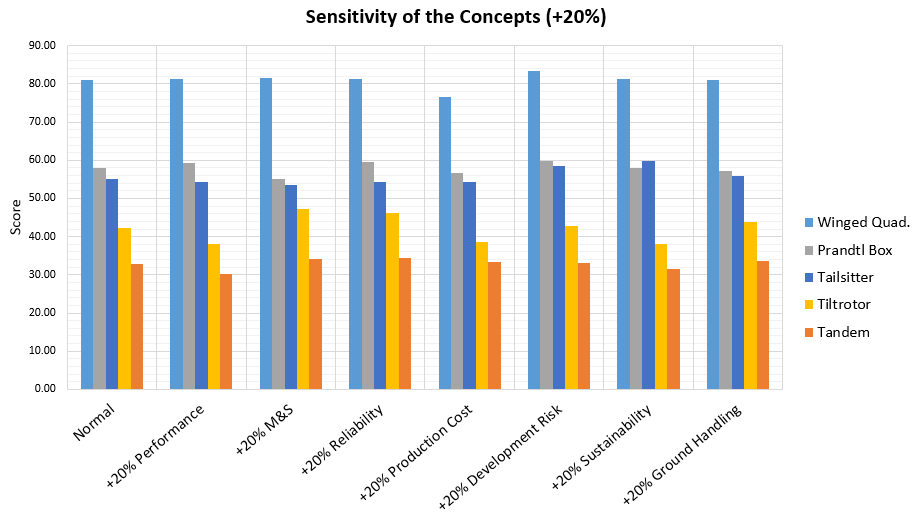
\includegraphics[width=\textwidth]{ConceptTradeOff/Figures/sensitivity}
    \caption{Sensitivity Analysis of the Final Trade-off}
    \label{fig:sensitivityanal}
\end{figure}

The figure shows that even thought the weights of the criteria are changed, The Wing Quadcopter scores highest every time. The gap between the first best and second best does not decrease drastically during the sensitivity analysis, showing that the weighting will not influence the end results. The overall rankings of the concepts also remain unchanged everywhere except when sustainability is weighted 20\% more, this is because The Tailsitter scores 26 higher than The Prandtl Box for that criterion.

Since the Winged Quadcopter greatly outperforms all other concepts throughout the entire sensitivity analysis, it is safe to say that this concept has the greatest potential to satisfy all requirements. Therefore it is sensible to further develop this concept into the preliminary design phase.


\section{Concept Analysis}
\label{sec:conc_anal}
%Technical Risk Assessment


